\documentclass[letterpaper]{article}
\usepackage[margin=1in]{geometry}
\usepackage[utf8]{inputenc}
\usepackage{textcomp}
\usepackage{amssymb}
\usepackage{natbib}
\usepackage{graphicx}
\usepackage{gensymb}
\usepackage{amsthm, amsmath, mathtools}
\usepackage[dvipsnames]{xcolor}
\usepackage{enumerate}
\usepackage{mdframed}
\usepackage[most]{tcolorbox}
\usepackage{csquotes}
% https://tex.stackexchange.com/questions/13506/how-to-continue-the-framed-text-box-on-multiple-pages

\tcbuselibrary{theorems}

\newcommand{\R}{\mathbb{R}}
\newcommand{\Z}{\mathbb{Z}}
\newcommand{\N}{\mathbb{N}}
\newcommand{\Q}{\mathbb{Q}}
\newcommand{\C}{\mathbb{C}}
\newcommand{\code}[1]{\texttt{#1}}
\newcommand{\mdiamond}{$\diamondsuit$}
\newcommand{\PowerSet}{\mathcal{P}}
\newcommand{\Mod}[1]{\ (\mathrm{mod}\ #1)}
\DeclareMathOperator{\lcm}{lcm}

%\newtheorem*{theorem}{Theorem}
%\newtheorem*{definition}{Definition}
%\newtheorem*{corollary}{Corollary}
%\newtheorem*{lemma}{Lemma}
\newtheorem*{proposition}{Proposition}


\newtcbtheorem[number within=section]{theorem}{Theorem}
{colback=green!5,colframe=green!35!black,fonttitle=\bfseries}{th}

\newtcbtheorem[number within=section]{definition}{Definition}
{colback=blue!5,colframe=blue!35!black,fonttitle=\bfseries}{def}

\newtcbtheorem[number within=section]{corollary}{Corollary}
{colback=yellow!5,colframe=yellow!35!black,fonttitle=\bfseries}{cor}

\newtcbtheorem[number within=section]{lemma}{Lemma}
{colback=red!5,colframe=red!35!black,fonttitle=\bfseries}{lem}

\newtcbtheorem[number within=section]{example}{Example}
{colback=white!5,colframe=white!35!black,fonttitle=\bfseries}{def}

\newtcbtheorem[number within=section]{note}{Important Note}{
        enhanced,
        sharp corners,
        attach boxed title to top left={
            xshift=-1mm,
            yshift=-5mm,
            yshifttext=-1mm
        },
        top=1.5em,
        colback=white,
        colframe=black,
        fonttitle=\bfseries,
        boxed title style={
            sharp corners,
            size=small,
            colback=red!75!black,
            colframe=red!75!black,
        } 
    }{impnote}
\usepackage[utf8]{inputenc}
\usepackage[english]{babel}
\usepackage{fancyhdr}
\usepackage[hidelinks]{hyperref}

\pagestyle{fancy}
\fancyhf{}
\rhead{Math 100A}
\chead{September 14th, 2021}
\lhead{Course Notes}
\rfoot{\thepage}

\setlength{\parindent}{0pt}

\begin{document}

\begin{titlepage}
    \begin{center}
        \vspace*{1cm}
            
        \Huge
        \textbf{Math 100A Notes}
            
        \vspace{0.5cm}
        \LARGE
        Abstract Algebra
            
        \vspace{1.5cm}
            
        \vfill
            
        Fall 2021\\
        Taught by Professor Kiran Kedlaya
    \end{center}
\end{titlepage}

\pagenumbering{gobble}

\newpage 

\pagenumbering{gobble}
\begingroup
    \renewcommand\contentsname{Table of Contents}
    \tableofcontents
\endgroup

\newpage
\pagenumbering{arabic}

\section{Introduction to Binary Operations}
We want to explore the idea behind \emph{algebraic structures}. In particular, we want to explore these structures in more detail compared to earlier courses (either in past college or high school algebra classes). 


\bigskip 

To do this, we need to think about \emph{what} algebra really is. We might think about solving equations like $x^2 + 3x + 5 = 0$ for $x$. In particular, what is really happening here?

\bigskip 

Well, there are a couple of operations going on. Specifically, we have \emph{addition} and \emph{multiplication}. 
\[x \times x + 3 \times x + 5 = 0\]
We now want to examine these operations. Both of these operations $(+, \times)$ take in \underline{two numbers} and output \underline{one number}. The question we might have, then, is: how can we can generalize these operations?


\subsection{Binary Operations}
A \textbf{binary operation} is a way of taking in two values and outputting one value. Of course, we might now ask: what can these values be? These values can come from any specific set. 

\bigskip 

For example, we can consider addition over the integers ($\Z$). The sum of two integers is an integer. Similarly, we could consider multiplication over the integers. Again, the product of two integers is an integer. We could also consider multiplication or addition over the real, rational, or complex numbers. 

\bigskip 

The idea is that whatever ``type'' we give our binary operation, we will get that same ``type'' for our output. To formalize this, we have the following definition:  
\begin{definition}{Binary Operation}{}
    A binary operation (also known as the law of composition) consists of: 
    \begin{itemize}
        \item A set $S$. 
        \item An operation; more concretely, a function $S \times S \to S$.
    \end{itemize}

    More formally, a binary operation $*$ over a set $S$ is a function mapping $f: S \times S \to S$. For each $(a, b) \in S \times S$, we can denote the element $f(a, b)$ of $S$ by $a * b$.

    \bigskip 

    In this class, for $a, b \in S$, we will represent binary operations in one of several ways: 
    \begin{itemize}
        \item $ab$
        \item $f(a, b)$
        \item $a * b$
    \end{itemize}
\end{definition}

\textbf{Remark:}
\begin{itemize}
    \item An element $a \in S$ (where $S$ is a set equipped with a binary operation $*$) is \emph{invertible} if there is another element $b$ such that: 
    \[a * b = e \qquad b * a = 1\]
\end{itemize}


\subsubsection{Examples of Binary Operations}
Some common examples of binary operations are: 
\begin{itemize}
    \item $\Z$ under addition. 
    \item $\Z$ under subtraction. 
    \item $\Z$ under multiplication. 
    \item $\R$ under addition. 
    \item $\R$ under subtraction. 
    \item $\R$ under multiplication.
    \item $M_{2}$ ($\R$) under multiplication (here, $M_{2}$ denotes a $2 \times 2$ square matrix). 
    \item String concatenation.
\end{itemize}

\subsubsection{Non-Examples of Binary Operations}
One common non-example of a binary operation is $\R$ under division. This is because: 
\begin{itemize}
    \item Dividing a non-zero number by 0 (for example, $\frac{5}{0}$) produces undefined behavior. In other words, what is the result of this? 
    \item Dividing 0 by 0 is ambiguous. For example, this could be infinity, or it could be undefined. 
\end{itemize}
If we were to assume some value for a division-by-zero operation, then the operation would \textbf{not be closed}. That is, while we know that $0 \in \R$ and $n \in \R$ (denote $n$ to be any number in $\R$), we could say that $\frac{n}{0} = \infty$, but we know that $\infty \notin \R$, so the operation is not closed.  

\subsection{More on Binary Operations}
Anything that is ``like'' addition or multiplication is probably a binary operation. For example, let's consider \textbf{matrices}.
\begin{itemize}
    \item Addition of matrices of a fixed dimension. More specifically, the set of $n \times m$ matrices (here, $n$ and $m$ are fixed positive integers) over the integers, rationals, reals, or complex numbers under matrix addition is a binary operation.
    \[
        \begin{bmatrix}
            a_{11} & a_{12} & a_{13} \\ 
            a_{21} & a_{22} & a_{23}
        \end{bmatrix} + \begin{bmatrix}
            b_{11} & b_{12} & b_{13} \\ 
            b_{21} & b_{22} & b_{23}
        \end{bmatrix} = \begin{bmatrix}
            a_{11} + b_{11} & a_{12} + b_{12} & a_{13} + b_{13} \\ 
            a_{21} + b_{21} & a_{22} + b_{22} & a_{23} + b_{23}
        \end{bmatrix}
    \]

    \item Multiplication of matrices of a fixed dimension. More specifically, the set of $n \times n$ matrices (square matrices). We could also just multiply a $n \times m$ matrix by a $k \times l$ matrix assuming $m = k$ (otherwise, multiplying these two matrices will result in undefined behavior). 
\end{itemize}

So far, we considered binary operations on infinite sets in which we need some sort of formula to describe (e.g. $f_{\cup}(A, B) = A \cup B$). Now, if we have a finite set, we could define a binary operation exhaustively by just saying what the binary operation does on every pair of entries.

\bigskip 

For example, given the set $S = \{a, b, c, d, e\}$. We can define a binary operation on $S$ with the below \textbf{function table}: 
\begin{center}
    \begin{tabular}{c | c c c c c}
            & $a$ & $b$ & $c$ & $d$ & $e$ \\ 
        \hline 
        $a$ & $a$ & $c$ & $d$ & $d$ & $e$ \\ 
        $b$ & $b$ & $c$ & $c$ & $b$ & $a$ \\ 
        $c$ & $d$ & $e$ & $e$ & $b$ & $b$ \\ 
        $d$ & $a$ & $a$ & $a$ & $c$ & $a$ \\ 
        $e$ & $b$ & $b$ & $c$ & $c$ & $d$
    \end{tabular}
\end{center}
Denote the binary operation to be $\#$.
\begin{itemize}
    \item What is $c \# d$? The answer is $b$. 
    \item What is $e \# ((a \# b) \# c)$? The answer is $d$.
    \item Suppose we have $X \# a = a$. What is $X$? The answer is $X = a, d$.
\end{itemize}

\subsection{Properties of Binary Operations}
What properties could binary operations have?

\begin{itemize}
    \item \textbf{Commutativity:} A binary operation is commutative if the order of the two inputs does not matter. For example, if $f$ is a function corresponding to a binary operation, then:
    \[f(a, b) = f(b, a) \quad \forall a, b \in S\] 
    More commonly:
    \[a * b = b * a \quad \forall a, b \in S\]

    For example, addition or multiplication of numbers is commutative. Unions and intersections of sets is also commutative. \emph{However}, matrix multiplication is \emph{not} commutative. Our example above is also not commutative. 

    \item \textbf{Associativity:} A binary operation is associative if the order of applying the operation (in a string) does not matter. Specifically:
    \[(a * b) * c = a * (b * c) \quad \forall a, b, c \in S\]
    Which means that we can write $a * b * c$ (or even $abc$) without ambiguity.
    
    \bigskip 

    For example, addition or multiplication of numbers is associative. Addition or multiplication of matrices is also associative. Our example above is not associative. 

    \item \textbf{Identity:} A binary operation has a two-sided identity element and a two-sided inverse for every element. 
    
    \bigskip 
    
    More specifically, we say that $e$ is a left identity if $f(e, s) = s$ for all $s \in S$. $e$ is a right identity if $f(s, e) = s$ for all $s \in S$. Then, $e$ is a two-sided identity if it is both a left identity and right identity.  
    
    \bigskip 

    For example, 0 is a two-sided identity for addition and 1 is a two-sided identity for multiplication. For matrix addition, the zero-matrix is a two-sided identity. For matrix multiplication, the matrix with ones on the diagonal and zeros everywhere else is the identity element. In our example above, $\#$ does not have a left or right identity. 

    \bigskip 

    As a fact, there can be \textbf{at most} one identity element for any given binary operation. The proof is discussed later. 

    \item \textbf{Inverse:} For a general \underline{associative} binary operation $f: S \times S \to S$ with a two-sided identity $e$, an element $s \in S$ has a two-sided inverse if it has a left inverse (denote this $l \in S$) and a right inverse (denote this $r \in S$); that is: 
    \[\overbrace{f(l, s)}^{\text{Left Inverse}} = \underbrace{f(s, r)}_{\text{Right Inverse}} = e\]

    \bigskip 

    We often write $s^{-1}$ to mean an inverse of $s$ when it exists. So, for instance (both ways are the same thing), we could have written: 
    \[f(s^{-1}, s) = f(s, s^{-1}) = e\]
    \[s^{-1} * s = s * s^{-1} = e\]

    \bigskip 

    There are several common examples. In addition, this is the negative/negation. In other words, the additive inverse of $x$ is $-x$. In multiplication, this is the reciprocal. The multiplicative inverse of $x$ is $\frac{1}{x}$ (for all $x \neq 0$). 
    
    \bigskip 
    
    Several facts to keep in mind: 
    \begin{itemize}
        \item Any element has at most one inverse. 
        \item An element with a left inverse and a right inverse also has an inverse (this was shown above). 
        \item If every element has an inverse and the binary operation (or composition) is associative, then the cancellation property holds: 
        \[a * b = a * c \implies b = c\]
        \[b * a = c * a \implies b = c\]
    \end{itemize}
\end{itemize}

\textbf{Remark:} Commutativity does not imply associativity.

\newpage 
\section{Groups}
Of course, the properties of binary operations that were discussed just now are very much applicable in something called \textbf{groups}. Simply put, we can say that a group is a set combined with an operation. However, it's a little more complicated than that. The following definition will make that clearer:
First, we show that\begin{definition}{Group}{}
    A group is a set $G$, closed under a binary operation $*$, satisfying the following properties:
    \begin{enumerate}
        \item \underline{Associativity}: For all $a, b, c \in G$, we have:
        \[(a * b) * c = a * (b * c)\]

        \item \underline{Identity/Neutral Element:} There is an element $e \in G$ such that for all $x \in G$:
        \[e * x = x * e = x\]

        \item \underline{Inverse:} Corresponding to each $a \in G$, there is an element $a^{-1} \in G$ such that:
        \[a * a^{-1} = a^{-1} * a = e\]

        \item \underline{Closure:} For all $a, b \in G$, we have:
        \[a * b \in G\]
        It should be noted that this property is \emph{implied} by the definition of a binary operation (law of composition); namely, that $G \times G \to G$.  
    \end{enumerate}
\end{definition}
\textbf{Remark:}
\begin{itemize}
    \item Notationally, this can be represented by $(G, *)$ or $\langle G, * \rangle$. This is saying that we are pairing a set with a binary operation. 
\end{itemize}

\begin{definition}{Abelian Group}{}
    A group is \textbf{abelian} if it is commutative.
\end{definition}
\textbf{Remark:}
\begin{itemize}
    \item Recall that a group is commutative if applying the group operation to two group elements does not depend on the order in which they are written. 
\end{itemize}

\begin{note*}{}{}
    The two most common groups are additive and multiplicative groups. Thus, for some $h \in G$, where $(G, *)$ is a group, it is important to mention what their inverses and identity elements are. As mentioned in the previous section:
    \begin{center}
        \begin{tabular}{|c|c|c|}
            \hline 
            \textbf{Group} & \textbf{Inverse} & \textbf{Identity} \\ 
            \hline 
            Multiplicative $(G, \times)$ & $h^{-1} = \frac{1}{h}$ & $e = 1$ \\ 
            Addition $(G, +)$ & $h^{-1} = -h$ & $e = 0$ \\ 
            \hline 
        \end{tabular}
    \end{center}
    We will discuss these more in the examples. 

    \bigskip 

    For any other group, the inverse and identity element depends on how the group and its binary operation is defined. Refer to the definition of a group.
\end{note*}

\begin{note*}{}{}
    In \emph{Algebra, Second Edition} by Michael Artin, groups are denoted by the set followed by the binary operation (or law of composition) as the power. For example: 
    \begin{itemize}
        \item $\Z^+$ is the set of integers, with addition as its binary operation.
        \item $\R^+$ is the set of real numbers, with adition as its binary operation. 
        \item $\R^{\times}$ is the set of \underline{nonzero} real numbers, with multiplication as its binary operation.
    \end{itemize} 
\end{note*}

\subsection{Examples of Groups}
Here, we briefly describe some examples of groups. 

\subsubsection{Example: Addition}
For example, the integers under addition are a group. Notationally, this is represented by $(\Z, +)$. 
\begin{itemize}
    \item It's obvious that addition is associative. That is:
    \[(a + b) + c = a + (b + c) = a + b + c\]

    \item The identity element is 0 (we note that $0 \in \Z$). This is because:
    \[0 + x = x + 0 = x\]

    \item The inverse is $-x$. This is because:
    \[x + (-x) = (-x) + x = 0\]
\end{itemize}
We also know that the reals, rationals, or complex numbers under addition are also groups. Notationally, this is represented by $(\R, +)$, $(\Q, +)$, or $(\C, +)$, respectively. 

\bigskip 

Additionally, these are all considered to be \textbf{abelian groups}. 

\subsubsection{Example: Multiplication}
Let's now consider multiplication. In particular, multiplication does give a binary operation over $\Z$, $\Q$, $\R$, and $\C$. It's obvious that this is associative and 1 is the two-sided identity element. However, what about the inverse? 
\begin{itemize}
    \item If we try to take the integers under multiplication as a group, then we'll run into problems. This is because the multiplicative inverse of every \underline{integer} except $\pm 1$ is not an integer. For example, if we tried 2, then the multiplicative inverse of 2 is $\frac{1}{2}$. However, $\frac{1}{2} \notin \Z$.
    
    \item Rational numbers are closer. For instance, $\left(\frac{a}{b}\right)^{-1} = \frac{b}{a}$. However, this is only defined if $a \neq 0$. The solution is to remove 0. So, $(\Q - \{0\}, \times)$ is a group. Similarly, we can make $\R$ and $\C$ groups under multiplication by removing 0. 
    
    \bigskip 

    We note that this change does not affect the closure property because we can only achieve $a \times b = 0$ if and only if $a = 0$ or $b = 0$. Since $a \notin \R - \{0\}$ and $b \notin \R - \{0\}$ (or $\Q$ or $\C$), then we are still closed and our binary operation is still well-defined. 
\end{itemize}

\subsubsection{Example: Matrices}
Consider the $n \times n$ general linear group, or the group of all invertible\footnote{Here, keep in mind that the determinant of an invertible matrix is not 0 (otherwise, it wouldn't have an inverse.)} $n \times n$ matrices. This is denoted by: 
\[GL_n = \{n \times n \text{ invertible matrices } A\}\]
If we wanted to indicate that we are working with real or complex matrices, we write $GL_{n}(\R)$ and $GL_{n}(\C)$, respectively.

\subsubsection{Non-Example: Addition and Multiplication}
We mentioned that $(\Q - \{0\}, \times)$, $(\R - \{0\}, \times)$, and $(\C - \{0\}, \times)$ are groups. However, we note that $(\Z - \{0\}, \times)$ and $(\Z_{\geq 0}, +)$ are \emph{not} groups. 
\begin{itemize}
    \item We already briefly explained why $\Z$ under multiplication is not a group. The same idea applies even if we do not include 0; that is, $\Z - \{0\}$ is not a group. We know that $\Z - \{0\}$ has a unique identity element under $\times$; this element is 1. This is the case because, if $e$ is the identity element of $\Z - \{0\}$ under $\times$, then by definition: 
    \[e \times x = x \times e = x\]
    Which implies that $e = 1$. We also know that $2 \in \Z - \{0\}$. However, 2 does not have an inverse in $\Z - \{0\}$. To show this, we prove by contradition. If 2 has an inverse in $\Z - \{0\}$, then by definition it follows that for some $a^{-1} \in \Z - \{0\}$:
    \[2 \times a^{-1} = a^{-1} \times 2 = e\]
    But, since we know that $e = 1$, it follows that:
    \[2 \times a^{-1}= 1\]
    But, as the only solution to this is $\frac{1}{2}$, we know that $\frac{1}{2} \notin \Z - \{0\}$. Thus, this is a contradiction. Thus, $\Z - \{0\}$ under multiplication is not a group. 

    \item We know that $\Z_{\geq 0}$ has a unique identity element under addition and that is 0. This is because if $e$ is a unique element of $(\Z_{\geq 0}, +)$, then by definition, we know that: 
    \[e + x = x + e = x\]
    It is obvious that $e = 0$. Now, we want to show that 1 does not have an inverse with respect to addition in $\Z_{\geq 0}$. We'll prove this by contradiction. Suppose 1 does have an inverse. Recall that if 1 does have an inverse, then there is an $x \in \Z_{\geq 0}$ such that for some $a^{-1} \in \Z_{\geq 0}$:
    \[a^{-1} + 1 = 1 + a^{-1} = e\]
    But, as $e = 0$, it follows that: 
    \[a^{-1} + 1 = 0 \iff a^{-1} = -1\]
    However, we note that $-1 \notin \Z_{\geq 0}$ so this is a contradiction. Thus, $\Z_{\geq 0}$ under addition is not a group.
\end{itemize}

\subsection{Basic Properties of Groups}
Suppose $(G, *)$ is a group. Then, we note the following properties of groups. 

\subsubsection{Uniqueness of the Identity.} 
Could we have two unique two-sided identities in $G$? The answer is \underline{no}. The proof is as follows. 

\begin{mdframed}
    \begin{proof}
        Assume by contradiction that we had $e_1$ and $e_2$, both of which are unique two-sided identity elements. Then, we know that $e_1 * e_2 = e_2$ since $e_1$ is an identity. But, since $e_2$ is also an identity, then $e_1 * e_2 = e1$. So, it follows that $e_1$ and $e_2$ are not unique; in other words, $e_1 = e_2$. 
    \end{proof}
\end{mdframed}

\subsubsection{Uniqueness of Inverses.}

If $g_1$, $g_2$ are both inverses of some element $h$, then\footnote{Here, we denote $g_1$ as the left-inverse and $g_2$ is the right-inverse.}:
\[g_1 * h = h * g_2 = e\]
Additionally, we know that:
\[g_1 * (h * g_2) = g_1 * e = g_1\]
\[(g_1 * h) * g_2 = e * g_2 = g_2\]
And so it follows that $g_1 = g_2$, thus $h$ will have a unique inverse. To be more concrete, we have the proof. 
\begin{mdframed}
    \begin{proof}
        We note that $g_1 * h = e$ and $h * g_2 = e$. Then:
        \begin{equation*}
            \begin{aligned}
                g_1 &= g_1 * e && e \text{ is the identity element.} \\ 
                    &= g_1 * (h * g_2) \\ 
                    &= (g_1 * h) * g_2 && \text{Associativity} \\ 
                    &= e * g_2 \\ 
                    &= g_2 && e \text{ is the identity element.}
            \end{aligned}
        \end{equation*}
        So, it follows that $g_1 = g_2$. Thus, an element $h$ will have a unique inverse. 
    \end{proof}
\end{mdframed}

\subsubsection{Cancellation.}
Suppose we have the expression $g * a = g * b$. This implies that $a = b$. Similarly, the expression $a * g = b * g$ can be simplified to $a = b$. 

\begin{mdframed}
    \begin{proof}
        From the definition of a group, we know that an inverse exists for every element in $G$. Let $g^{-1}$ be the inverse of $g$. Then:
        \begin{equation*}
            \begin{aligned}
                g * a = g * b &\implies g^{-1} * (g * a) = g^{-1} * (g * b) \\
                    &\implies (g^{-1} * g) * a = (g^{-1} * g) * b && \text{Associativity (Prop. 1)} \\
                    &\implies e * a = e * b && \text{Definition of Inverse (Prop. 3)} \\  
                    &\implies a = b && \text{Definition of Identity (Prop. 2)}
            \end{aligned}
        \end{equation*}
        The other way is similar. 
    \end{proof}
\end{mdframed}

\textbf{Remark:} Although $g * a = g * b$, $g * a \neq b * g$ ($g * a$ is not necessarily equal to $b * g$). 

\subsubsection{Inverse of Operation of Two Elements.}

\begin{lemma}{}{}
    Suppose $(G, *)$ is a group. Then, for every $g, h \in G$, we have: 
    \[(g * h)^{-1} = h^{-1} * g^{-1}\]
\end{lemma}

\begin{mdframed}
    \begin{proof}
        Since the inverse of an element is unique, it is enough to check that: 
        \[(g * h) * (h^{-1} * g^{-1}) = (h^{-1} * g^{-1}) * (g * h) = e\]
        So: 
        \begin{equation*}
            \begin{aligned}
                (g * h) * (h^{-1} * g^{-1}) &= g * (h * h^{-1}) * g^{-1} && \text{Associativity (Prop. 1)} \\ 
                    &= g * e * g^{-1} && \text{Definition of Inverse (Prop. 3)} \\ 
                    &= (g * e) * g^{-1} && \text{Associativity (Prop. 1)} \\ 
                    &= g * g^{-1} && \text{Definition of Identity (Prop. 2)} \\ 
                    &= e && \text{Identity Element}
            \end{aligned}
        \end{equation*}
        Similarly: 
        \begin{equation*}
            \begin{aligned}
                (h^{-1} * g^{-1}) * (g * h) &= h^{-1} * (g^{-1} * g) * h && \text{Associativity (Prop. 1)} \\ 
                    &= h^{-1} * e * h && \text{Definition of Inverse (Prop. 3)} \\ 
                    &= (h^{-1} * e) * h && \text{Associativity (Prop. 1)} \\ 
                    &= h^{-1} * h && \text{Definition of Identity (Prop. 2)} \\ 
                    &= e && \text{Identity Element}
            \end{aligned}
        \end{equation*}
        So, the proof is complete. 
    \end{proof}
\end{mdframed}

\subsubsection{Inverse of an Inverse.}
We should note that, despite using the $-1$ superscript to denote a multiplicative inverse, this applies to any valid binary operation under a group. 

\begin{lemma}{}{}
    For every $g \in G$, $(g^{-1})^{-1} = g$. 
\end{lemma}

\begin{mdframed}
    \begin{proof}
        We have that $g^{-1} * g = e$. Multiplying both sides by $(g^{-1})^{-1}$ from the left, we now have: 
        \[((g^{-1})^{-1} * g^{-1}) * g = (g^{-1})^{-1} * e = (g^{-1})^{-1}\]
        Hence, $e * g = (g^{-1})^{-1}$ and so $g = (g^{-1})^{-1}$.     
    \end{proof}
\end{mdframed}

\subsection{Exponents of Elements}
Suppose $(G, *)$ is a group and $g \in G$. For a positive integer $n$, we let: 
\[g^n = \underbrace{g * \dots * g}_{n \text{ times}}\]
For a negative integer $n$, we let: 
\[g^n = \underbrace{(g^{-1}) * \dots * (g^{-1})}_{-n \text{ times}}\]

\begin{lemma}{}{}
    For $n, m \in \Z$, $(g^n)^m = g^{nm}$. 
\end{lemma}

\begin{mdframed}
    \begin{proof}
        We will consider various cases depending on the signs of $m$ and $n$. 
        \begin{itemize}
            \item \underline{Case 1:} Suppose $m$ and $n$ are positive. Then: 
            \[(g^n)^m = \underbrace{g^n * \dots * g^n}_{m \text{ times}} = \underbrace{\overbrace{(g * \dots * g)}^{n \text{ times}} * \dots * \overbrace{(g * \dots * g)}^{n \text{ times}}}_{m \text{ times}} = \underbrace{g * \dots * g}_{mn \text{ times}} = g^{mn}\]
            Here, $g^n$ means we need to multiply $g$ $n$ times. But, since we need to multiply $g^n$ $m$ times, it follows that this is simply $g^{nm}$.  

            \item \underline{Case 2:} Suppose $m$ is positive and $n$ is negative. Then: 
            \[(g^n)^m = \underbrace{g^n * \dots * g^n}_{m \text{ times}} = \underbrace{\overbrace{(g^{-1} * \dots * g^{-1})}^{-n \text{ times}} * \dots * \overbrace{(g^{-1} * \dots * g^{-1})}^{-n \text{ times}}}_{m \text{ times}} = \underbrace{g^{-1} * \dots * g^{-1}}_{-mn \text{ times}} = g^{mn}\]
            Here, we note that $mn < 0$. 

            \item \underline{Case 3:} Suppose $m$ is negative and $n$ is positive. Then: 
            \[(g^n)^m = \underbrace{(g^n)^{-1} * \dots * (g^n)^{-1}}_{-m \text{ times}} = \underbrace{(\overbrace{g * \dots * g}^{n \text{ times}})^{-1} * \dots * (\overbrace{g * \dots * g}^{n \text{ times}})^{-1}}_{-m \text{ times}}\]

            We note that, by the previous lemma, $(\underbrace{g * \dots * g}_{n \text{ times}})^{-1} = \underbrace{g^{-1} * \dots * g^{-1}}_{n \text{ times}}$. Hence: 
            \[(g^n)^m = \underbrace{(\overbrace{g^{-1} * \dots * g^{-1}}^{n \text{ times}}) * \dots * (\overbrace{g^{-1} * \dots * g^{-1}}^{n \text{ times}})}_{-m \text{ times}} = \underbrace{g^{-1} * \dots * g^{-1}}_{-mn \text{ times}} = g^{mn}\]
            Here, we note that $mn < 0$.  

            \item \underline{Case 4:} Suppose $m$ and $n$ are negative. Since it is easier to work with positive numbers, let $m = -r$ and $n = -s$ where $r, s > 0$. Then, we have to show that $(g^{-r})^{-s} = g^{rs}$. By definition, we know that $g^{-r} = \underbrace{g^{-1} * \dots * g^{-1}}_{r \text{ times}}$. Hence, $(g^{-r})^{-s} = [(g^{-1})^r]^{-s}$. By the case where $n > 0$ and $m < 0$, we deduce that $(x^r)^{-s} = x^{-rs}$. Therefore: 
            \[(g^{-r})^{-s} = (g^{-1})^{-rs} = \underbrace{(g^{-1})^{-1} * \dots * (g^{-1})^{-1}}_{rs \text{ times}} = \underbrace{g * \dots * g}_{rs \text{ times}} = g^{rs}\]

            \item \underline{Case 5:} Suppose $m = 0$. Since $m = mn = 0$, it follows that: 
            \[(g^n)^m = e\]
            \[g^{nm} = e\]

            \item \underline{Case 6:} Suppose $n = 0$. By the same reasoning as case 5, we have that $n = mn = 0$. So: 
            \[(g^n)^m = e^m = e\]
            \[g^{mn} = e\]
        \end{itemize}

        Here, we notice that $e * \dots * e = e$ and $e^{-1} = e$, and so $e^m = e$. So, we showed that $(g^n)^m = g^{mn}$ for every $m, n \in \Z$. 
    \end{proof}
\end{mdframed}

\begin{note*}{}{}
    \begin{itemize}
        \item When we are working with an \underline{multiplicative group} $(G, \times)$, then $g^n$ means:
        \[g^n = \begin{cases}
            \underbrace{g \times \dots \times g}_{n \text{ times}} & n > 0 \\ 
            1 & n = 0 \\ 
            \underbrace{\frac{1}{g} \times \dots \times \frac{1}{g}}_{-n \text{ times}} & n < 0
        \end{cases}\]

        \item When we are working with an \underline{additive group} $(G, +)$, instead of writing $g^n$, we write $ng$. So, in $(G, +)$: 
        \[ng = \begin{cases}
            \underbrace{g + \dots + g}_{n \text{ times}} & n > 0 \\ 
            0 & n = 0 \\ 
            \underbrace{(-g) + \dots + (-g)}_{-n \text{ times}} & n < 0
        \end{cases}\]
        So, instead of writing $(g^{n})^m = g^{mn}$, we write $m(ng) = (mn)g$.

        \item For other valid groups, it depends on how you define the operation for the group. 
    \end{itemize}
\end{note*}

\begin{lemma}{}{}
    For every $m, n \in \Z$: 
    \[g^m * g^n = g^{m + n}\]
\end{lemma}

\begin{mdframed}
    \begin{proof}
        Like the previous proof, we will consider various cases depending on the signs of $m$ and $n$. Since it is easier to work with positive numbers, we will write $m = \text{sign}(m) r$ and $n = \text{sign}(n) s$ where $r = |m|$ and $s = |n|$, where: 
        \[\text{sign}: \R \to \{-1, 1\}\]
        \begin{itemize}
            \item \underline{Case 1:} Suppose $m$ and $n$ are positive. Then: 
            \[g^m * g^n = (\underbrace{g * \dots * g}_{m \text{ times}}) * (\underbrace{g * \dots * g}_{n \text{ times}}) = \underbrace{g * \dots * g}_{m + n \text{ times}} = g^{m + n}\]
    
            \item \underline{Case 2:} Suppose $m = -r$ ($m$ is negative), $n = s$ ($n$ is positive), $r < s$ ($m + n$ is positive). Then, by the previous case:
            \[g^r * g^{s - r} = g^s \implies g^{s - r} = (g^r)^{-1} * g^s = g^{-r} * g^s\]  
    
            \item \underline{Case 3:} Suppose $m = -r$, $n = s$, $r > s$ ($m + n$ is negative). Then, by the first case: 
            \begin{equation*}
                \begin{aligned}
                    g^s * g^{r - s} = g^r &\implies g^{r - s} = (g^s)^{-1} * g^r \\ 
                        &\implies (g^{r - s})^{-1} = ((g^s)^{-1} * g^r)^{-1} \\ 
                        &\implies g^{-(r - s)} = (g^r)^{-1} * ((g^s)^{-1})^{-1} \\ 
                        &\implies g^{-r + s} = g^{-r} * g^s
                \end{aligned}
            \end{equation*}
    
            \item \underline{Case 4:} Suppose $m = 0$. Then: 
            \[g^m * g^n  = e * g^n = g^n = g^{m + n}\]
    
            \item \underline{Case 5:} Suppose $n = 0$. Then: 
            \[g^m * g^n = g^m * e = g^m = g^{m + n}\]
        \end{itemize}
        By the above cases, we obtain the claim when $n \geq 0$ and $m \in \Z$. So: 
        \begin{itemize}
            \item \underline{Case 6:} Suppose $n = -s$ ($n$ is negative) and $s > 0$. Then: 
            \[g^{m - s} * g^s = g^m \implies g^{m - s} = g^m * (g^s)^{-1} \implies g^{m - s} = g^m * g^{-s}\]
        \end{itemize}
        This concludes the proof. 
    \end{proof}
\end{mdframed}

\newpage 
\section{Subgroups}
The definition of a subgroup is very similar to that of a group. It states the following. 
\begin{definition}{Subgroup}{}
    A subset $H$ of a group $G$ is a \textbf{subgroup} if it has the following properties: 
    \begin{enumerate}
        \item \underline{Identity/Neutral Element:} The identity element of $G$ belongs in $H$. In other words, there is an element $e \in H$ (where the same $e \in G$) such that for all $x \in H$:
        \[e * x = x * e = x\]

        \item \underline{Inverse:} For some $a \in H$, its inverse in $G$ belongs to $H$. More generally, corresponding to each $a \in H$, there is an element $a^{-1} \in H$ such that:
        \[a * a^{-1} = a^{-1} * a = e\]

        \item \underline{Closure:} For all $a, b \in H$, we have:
        \[a * b \in H\]
        It should be noted that this property is \emph{implied} by the definition of a binary operation (law of composition). This binary operation is inherited from the group $G$.  
    \end{enumerate}
\end{definition}
\textbf{Remarks:}
\begin{itemize}
    \item Because associativity is a property that is in a group, it is also implicitly a property that is in a subgroup. 
    \item This also implies that the subgroup $H$ is a group.
    \item If $G$ is a group, then $G$ is a subgroup of itself. If we want to exclude this property (i.e. we don't want $G$ to be classified as a subgroup of itself), we would want $H$ to be a \emph{proper subgroup} of $G$.
    \item The identity element $\{e\}$ by itself is known as a \emph{trivial subgroup}. 
\end{itemize}


\subsection{Examples of Subgroups}
Here, we briefly describe some examples of subgroups. 

\subsubsection{Example: Complex Numbers Under Multiplication}
Consider the group $\C^{\times} = (\C - \{0\}, \times)$. $\{z \in \C \mid |Z| = 1\}$ (the set of all elements of the complex plane with absolute value 1) is a subgroup of $(\C - \{0\}, \times)$. 

\subsubsection{Example: Matrices}
Consider the set $GL_{n}(\R)$, or the set of all $n \times n$ invertible matrices, under matrix multiplication. Then, define: 
\[SL_{n}(\R) = \{A \in GL_{n}(\R) \mid \det(A) = 1\}\]
We have that $SL_{n}(\R)$ is a subgroup of $GL_{n}(\R)$. 

\subsubsection{Example: Real Numbers Under Addition}
Consider the group $(\R, +)$. Some possible subgroups are: 
\begin{itemize}
    \item $(\Z, +)$. The group of integers under addition. 
    \item $(\Z a, +)$. Here, we note that:
    \[(\Z a, +) = \{n \in Z \mid n = ka \text{ for some } k \in \Z\}\]
    \item $(\{0\}, +)$. The trivial subgroup, consisting of only the identity element.
    \item $(\R, +)$. The whole group. 
\end{itemize}

Effectively, a subgroup $H$ of a group $G$ with law of composition written \textbf{additively} is a subgroup if it has the following properties: 
\begin{itemize}
    \item \textbf{Closure:} If $a, b \in H$, then $a + b \in H$. 
    \item \textbf{Identity:} $0 \in H$. 
    \item \textbf{Inverses:} If $a \in S$, then $-a \in S$. 
\end{itemize}

\subsubsection{Example: Integers Under Addition}
Consider the group $(\Z, +)$. Some subgroups include: 
\begin{itemize}
    \item $(\{0\}, +)$: the trivial subgroup.
    \item $(\Z, +)$: the group itself.
    \item $(\Z 2, +)$: the group where the set is all even integers. 
    \item $(\Z a, +)$. The group where the set consists of all elements that is divisible by $a$. That is: 
    \[(\Z a, +) = \{n \in Z \mid n = ka \text{ for some } k \in \Z\}\] 
\end{itemize}

\subsection{More on Subgroups}
Of course, we now need to discuss some theorems and applications of subgroups. 
\begin{theorem}{}{}
    Let $S$ be a subgroup of the additive group $(\Z, +)$. Either $S$ is the trivial subgroup $\{0\}$, or else it has the form $\Z a$, where $a$ is the smallest positive integer in $S$. 
\end{theorem}

\begin{mdframed}
    \begin{proof}
        Let $S$ be a subgroup of $(\Z, +)$. Then, by definition, $0 \in S$. If 0 is the only element of $S$, then $S$ is the trivial subgroup and we are done. 

        \bigskip 

        Otherwise, $S$ contains an integer $n$ that is different from 0, and either $n$ or $-n$ is positive. We know that $-n \in S$ (inverse property) so, in either case, $S$ has a positive integer. Now, we need to show that $S$ is equal to $\Z a$ when $a$ is the smallest positive integer in $S$. 

        \bigskip 

        First, we show that $\Z a \subseteq S$; in other words, that $ka$ is in $S$ for every integer $k$. If $k$ is a positive integer, then $ka = \underbrace{a + a + \dots + a}_{k \text{ times}}$. Since $a \in S$, closure and induction shows us that $ka \in S$. Since inverses are in $S$, $-ka \in S$. Finally, $0 = 0a \in S$. 

        \bigskip 

        To show $\Z a = S$, assume by contradiction that it's not. Pick some $n \in S$ with $n \notin \Z a$. By Euclidean division, $n = qa + r$ for some $q, r \in \Z$, where $0 \leq r < a$. Additionally, we cannot have $r = 0$ because $n \notin \Z a$. Then, $n \in S$ and $qa \in S$, $-qa \in S$, and therefore $n - qa = r \in S$. But, $r$ is positive and $r < a$, which is a contradiction. \qedhere 

        % Now, we need to show that $S \subseteq \Z a$; that is, every element $n$ of $S$ is an integer multiple of $a$. We can use division with remainder to write $n = qa + r$, where $q, r \in \Z$ and where the remainder $r$ is in the range $0 \leq r < a$. Since $\Z a$ is contained in $S$, $qa \in S$ and, of course, $n \in S$. Since $S$ is a subgroup, $r = n - qa \in S$. Now, by our choice, $a$ is the smallest positive integer in $S$, while the remainder $r$ is in the range $0 \leq r < a$. The only remainder that can be in $S$ is 0, so $r = 0$ and $n$ is the integer multiple $qa$ of $a$. 
    \end{proof}
\end{mdframed}

% prop 2.3.5

\newpage 
\section{Cyclic Groups} 
Here, we will briefly talk about cyclic groups, subgroups, and order of elements.

\subsection{Definitions}
\begin{definition}{Cyclic Subgroup}{}
    Let $G$ be a group. Let $x \in G$ be an element. A \textbf{cyclic subgroup} $H = \cyclic{x}$ generated by $x$ is the subset: 
    \[H = \{\dots, x^{-2}, x^{-1}, x^0, x^1, x^2, \dots\} \subseteq G\]
    Namely, we note that: 
    \[\cyclic{x} = \{x^n \mid x \in \Z\}\]
\end{definition}

To check that $H$ is a \underline{commutative} subgroup, we show that it meets the properties of a subgroup. In particular:  
\begin{itemize}
    \item \underline{Closure:} We have that (regardless of signs): 
    \[x^m x^n = x^{m + n}\]

    \item \underline{Identity:} We know that: 
    \[e = x^0 \in G\]

    \item \underline{Inverse:} We know that (regardless of signs): 
    \[x^n = x^{-n}\]
\end{itemize}

\textbf{Remark:} $H$ may or may not be infinite. For example, consider the group $(\Z, +)$. If $x = a$ (some positive integer), then the following is infinite: 
\[H = \Z a\]
However, if $x = 0$, then the following is finite: 
\[H = \{0\}\] 
Another example we can consider is the group $(\R - \{0\}, \times)$. Then, if $x = -1$, we have a group with two elements: 
\[H = \{1, -1\}\]
A final example we can consider for now is the group $(\C - \{0\}, \times)$. Then, if $x = i$, we have: 
\[H = \{1, i, -1, -i\}\]
By which it cycles around (hence the name). 

\begin{definition}{Cyclic Group}{}
    A group $(G, *)$ is called a \textbf{cyclic group} if $G = \cyclic{x}$ for some $x \in G$. 
\end{definition}

\subsection{Cyclic Groups are Abelian (Commutative)}
To show that cyclic groups are abelian, we provide a proof. 
\begin{mdframed}
    \begin{proof}
        Suppose $(G, *)$ is cyclic. Then, $G = \cyclic{g}$ for some $g \in G$. Hence, $G = \{g^n \mid n \in \Z\}$. For every $x, y \in G$, there are integers $m$ and $n$ such that $x = g^m$ and $y = g^n$. Hence: 
        \[x * y = g^m * g^n = g^{m + n}\]
        \[y * x = g^n * g^m = g^{n + m}\]
        Since integers are abelian, it follows that $g^{n + m} = g^{m + n}$ so it follows that $x * y = y * x$.
    \end{proof}
\end{mdframed}

\subsection{Properties of Cyclic Subgroups}
Now, we'll talk about some important properties of cyclic subgroups.
\begin{theorem}{}{}
    Every subgroup of a cyclic group is cyclic.
\end{theorem}
The proof for this theorem is as follows: 
\begin{mdframed}
    \begin{proof}
        Suppose $(G, *)$ is generated by $g$ and $H$ is a subgroup of $G$. So, $G = \{g^n \mid n \in \Z\}$. If $H = \{e_G\}$, then it is generated by $e_G$ and so it is cyclic. Otherwise, we can assume (without loss of generality), we can and will assume that $H \neq \{e_G\}$. Hence, for some $l \in \Z - \{0\}$, $g^l \in H$. Because $H$ is a subgroup, we know that $(g^l)^{-1} \in H$. Thus, $g^{-l} \in H$. Either $l > 0$ or $-l > 0$, so there is a positive integer $m$ such that $g^m \in H$. By the well-ordering principle, there is: 
        \[s = \min\{m \in \Z \mid m > 0, g^m \in H\}\]
        Since $s \in \{m \in \Z \mid m > 0, g^m \in H\}$, it follows that $g \in H$. Because $H$ is a subgroup of $G$ and $g^r \in H$, $\cyclic{g^s} \subseteq H$. This implies that: 
        \[\{(g^s)^k \mid k \in \Z\} \subseteq H\]
        Which further implies that: 
        \[\{g^{sk} \mid k \in \Z\} \subseteq H\]
        Which completes this proof.
    \end{proof}
\end{mdframed} % TODO order discussed at 46:18

We now consider the following proposition.
\begin{mdframed}
    \begin{proposition}
        Let $\cyclic{x}$ be the cyclic subgroup of a group $G$ generated by an element $x$, and let $S \subseteq \Z$ denote the set of integer $k$ such that $x^k = 1$.
        \begin{enumerate}[(a)]
            \item The set $S$ is a subgroup of the additive group $(\Z, +)$ (closed under addition, contains 0, and closed under inverses). 
            \item Two powers $x^r = x^s$, with $r \geq s$, are equal if and only if $x^{r - s} = 1$; in other words, if and only if $r - s \in S$. 
            \item Suppose that $S$ is not the trivial subgroup. Then, $S = \Z n$ for some positive integer $n$. The powers $1, x, x^2, \dots, x^{n - 1}$ are the distinct elements of the subgroup $\cyclic{x}$, and the order of $\cyclic{x}$ is $n$. 
        \end{enumerate}
    \end{proposition}
\end{mdframed}

\textbf{Remarks:}
\begin{itemize}
    \item The order of $\cyclic{x}$ is the same thing as saying the cardinality of $\cyclic{x}$, or the number of elements. 
    \item An element $x \in G$ (a group) has order $n$ if $\cyclic{x}$ has order $n$. However, it's not correct to say that $x$ has a cardinality. 
    \item We can say that $x^n = 1$ and $x^r \neq 1$ for $r \in [1, \dots, n - 1]$. 
    \item For the third point, we can demonstrate this like so: 
    \[x^a = x^{qn + r} = (x^{n})^{q} x^r = 1^q x^r = x^r\]
    Essentially, it wraps around back to the identity element, so in that sense you can think of the exponents as the residue classes modulo $n$. 
    \item An element might have infinite order if it never cycles. 
\end{itemize}

\subsection{Examples of Cyclic Subgroups}
Here, we briefly explain some examples of cyclic subgroups.

\subsubsection{Example: Trivial}
The identity element, 1, has order 1. It cycles back immediately. 

\subsubsection{Example: Symmetric Group of Size 3}
Consider $G = S_3$. Then, we have: 
\begin{itemize}
    \item $x = (1 2)$: has order 2. 
    \item $x = (1 2 3)$: has order 3.
    \begin{itemize}
        \item $x^2 = (1 3 2)$
        \item $x^3 = (1)$
    \end{itemize}
\end{itemize}
Which elements of $S_3$ have order 6? 
\begin{itemize}
    \item $(1)$
    \item $(1 2)$
    \item $(2 3)$
    \item $(1 3)$
    \item $(1 2 3)$
    \item $(1 3 2)$
\end{itemize}
None of these elements have order 6, so $S_3$ is not a cyclic group. 

\subsubsection{Example: Matrices}
Consider $G = GL_{2}(\R)$. The element $x = \begin{bmatrix}
    1 & 1 \\ 
    0 & 1
\end{bmatrix}$ has infinite order. This is because: 
\[x^2 = \begin{bmatrix}
    1 & 2 \\ 
    0 & 1
\end{bmatrix}\]
\[x^3 = \begin{bmatrix}
    1 & 3 \\ 
    0 & 1
\end{bmatrix}\]
\[x^n = \begin{bmatrix}
    1 & n \\ 
    0 & 1
\end{bmatrix}\]

As you can see, we can never get back to the identity element. 

\subsubsection{Example: Matrices}
The matrix $x = \begin{bmatrix}
    1 & 1 \\ 
    -1 & 0
\end{bmatrix}$ has finite order. This is because: 
\[x^2 = \begin{bmatrix}
    0 & 1 \\ 
    -1 & -1
\end{bmatrix}\]
\[x^3 = \begin{bmatrix}
    -1 & 0 \\ 
    0 & -1
\end{bmatrix} = -I_2\]
\[x^4 = \begin{bmatrix}
    -1 & -1 \\ 
    1 & 0
\end{bmatrix} = -x\]
\[x^5 = \begin{bmatrix}
    0 & -1 \\ 
    1 & 1
\end{bmatrix} = -x^2\]
\[x^6 = \begin{bmatrix}
    1 & 0 \\ 
    0 & 1
\end{bmatrix} = I\]
So, $x$ has order 6. We note that $x^6 = x^0$. 

\subsection{More on Cyclic Groups}
Consider the following proposition: 
\begin{mdframed}
    \begin{proposition}
        Let $x \in G$ be an element of finite order $n$, and let $k$ be an integer that is written as $k = nq + r$ where $q$ and $r$ are integers and $r$ is in the range $0 \leq r < n$. Then: 
        \begin{itemize}
            \item $x^k = x^r$ 
            \item $x^k = 1$ if and only if $r = 0$
            \item Let $d$ be the greatest common divisor of $k$ and $n$. The order of $x^k$ is equal to $\frac{n}{d}$. 
        \end{itemize} 
    \end{proposition}
\end{mdframed}

For example, consider a cyclic group with order $n = 10$ and $k = 4$. Then: 
\[x^4, x^{2 \cdot 4}, x^{3 \cdot 4}, \dots, x^{m \cdot 4}\]
Here: 
\[4m \equiv 0 \Mod{10}\]
The smallest $m$ possible is: 
\[\frac{\lcm(n, k)}{k} = \frac{n}{\gcd(n, k)}\]

% 43:16









\newpage 
\section{Permutations}
Let's briefly discuss permutations, since these are important.
\begin{definition}{Permutation}{}
    A \textbf{permutation} of a set $S$ is a \underline{bijective map} $p$ from a set $S$ to itself: 
    \[p: S \to S\]
\end{definition}
For instance, consider the following table: 
\begin{center}
    \begin{tabular}{|c|c c c c c|}
        \hline 
        $i$ & 1 & 2 & 3 & 4 & 5 \\ 
        \hline 
        $p(i)$ & 3 & 5 & 4 & 1 & 2 \\ 
        \hline 
    \end{tabular}
\end{center}
This is a permutation $p$ of the set $\{1, 2, 3, 4, 5\}$. It is bijective because every element appears exactly once in the $p(i)$ row (i.e. we're only using each element once). In this particular table, there are two cycles:
\begin{itemize}
    \item Cycle 1: 
    \begin{itemize}
        \item $p(1) = 3$ (1 goes to 3)
        \item $p(3) = 4$ (3 goes to 4)
        \item $p(4) = 1$ (4 goes to 1)
    \end{itemize}
    \item Cycle 2: 
    \begin{itemize}
        \item $p(2) = 5$ (2 goes to 5)
        \item $p(5) = 2$ (5 goes to 2)
    \end{itemize}
\end{itemize}
If we drew this out, this would look like: 
\begin{verbatim}
    1 ---> 3
   /|\     |        5 ----> 2
    |     \|/      /|\      |
    |----- 4        |-------|
\end{verbatim}
This can be written in \textbf{cycle notation}:
\[p = (1 3 4)(2 5)\]
The first cycle $(1 3 4)$ is a 3-cycle and the second cycle $(2 5)$ is a 2-cycle\footnote{2-cycles are also known as \textbf{transpositions}.}.

\subsection{Symmetric Groups}
Now, we can introduce the notion of a symmetric group. 
\begin{definition}{Symmetric Group}{}
    For some $n \in \Z^+$, a \textbf{symmetric group} is the set of all permutations of the indices $\{1, 2, \dots, n\}$ and is denoted by $S_n$. 
\end{definition}
For instance, $S_3$ consists of the following permutations: 
\begin{itemize}
    \item $(123)$
    \item $(132)$
    \item $(21)$
    \item $(231)$
    \item $(312)$
    \item $(321)$
\end{itemize}

\subsection{Inverse of a Permutation}
Recall the permutation example used: 
\[p = (1 3 4)(2 5)\]
\begin{verbatim}
    1 ---> 3
   /|\     |        5 ----> 2
    |     \|/      /|\      |
    |----- 4        |-------|
\end{verbatim}








\newpage 
\section{Homomorphisms}
We will now discuss homomorphisms, which is one of the more important concepts to know.  

\subsection{Motivating Examples}
We begin the discussion of homomorphisms with two motivating examples.

\subsubsection{Motivating Example 1: Modulo Addition}
Let's suppose we are given two groups: 
\begin{itemize}
    \item \underline{Group 1:} $(\Z, +)$. 
    \item \underline{Group 2:} $(\Z / \Z 2, +)$.
\end{itemize}
These two groups may look completely unrelated at first. However, we note the following behaviors between the two groups:

\begin{center}
    \begin{tabular}{c|c}
        Operation in $(\Z, +)$ & Operation in $(\Z / \Z 2, +)$ \\ 
        \hline 
        Even + Even = Even. & $0 + 0 \equiv 0 \mod{2}$. \\ 
        Even + Odd = Odd. & $0 + 1 \equiv 1 \mod{2}$. \\ 
        Odd + Even = Odd. & $1 + 0 \equiv 1 \mod{2}$. \\ 
        Odd + Odd = Even. & $1 + 1 \equiv 0 \mod{2}$.
    \end{tabular}
\end{center}

Something to note here is that we can easily map:
\begin{itemize}
    \item \code{Even} (in first group) $\to$ \code{0} (in second group).
    \item \code{Odd} (in first group) $\to$ \code{1} (in second group).
\end{itemize}
This mapping can be represented like so: 
\[\phi: Z \to \Z / \Z 2\]
Where: 
\begin{itemize}
    \item If $x \in \Z$ is even, map it to $0 \in \Z / \Z 2$. 
    \item If $x \in \Z$ is odd, map it to $1 \in \Z / \Z 2$. 
\end{itemize}
Although these two groups appear to be completely unrelated, they are, in fact, related. 

\subsubsection{Example 2: Generalized Tables}
Suppose we have two groups $(G, *)$ and $(G', \cdot)$. They can be infinite, finite, commutative, non-commutative, etc. Suppose we have two elements $x, y \in G$. Then, we also know that $x * y \in G$ (closure). 

\bigskip 

Let's suppose we can represent the operations of the above group using a table, like so: 
\begin{itemize}
    \item \underline{Group 1:} $(G, *)$. Since we know that $x$, $y$, and $x * y \in G$, they'll appear in this table. 
    \begin{center}
        \begin{tabular}{|c|c c c|c|c|}
            \hline 
            $*$     & \dots & \dots & \dots & $y$     & \dots \\ 
            \hline 
            \vdots  &       &       &       &         &       \\ 
            \vdots  &       &       &       &         &       \\ 
            \hline 
            $x$     &       &       &       & $x * y$ &       \\ 
            \hline 
            \vdots  &       &       &       &         &       \\ 
            \vdots  &       &       &       &         &       \\ 
            \hline 
        \end{tabular}
    \end{center}

    \item \underline{Group 2:} $(G', \cdot)$. In order for these groups to have similar group behavior, $x$, $y$, and $x * y$ in $G$ must correspond to the elements in $G'$. This can be represented by a function: 
    \[\phi: G \to G'\]
    We want this function to send a specific part of the table for $G$ to a similar part of the table for $G'$. In this sense, we can say that the place where $x \in G$ is (in the above table) can be mapped to a similar place in the below table for $G'$; the same idea applies to $y \in G$ and $x * y \in G$.  
    \begin{center}
        \begin{tabular}{|c|c c c|c|c c|}
            \hline 
            $\cdot$   & \dots & \dots & \dots & $\phi(y)$      & \dots & \dots \\ 
            \hline 
            \vdots    &       &       &       &                &       &        \\ 
            \vdots    &       &       &       &                &       &        \\ 
            \hline 
            $\phi(x)$ &       &       &       & $\phi(x * y)$  &       &        \\ 
            \hline 
            \vdots    &       &       &       &                &       &        \\ 
            \vdots    &       &       &       &                &       &        \\ 
            \vdots    &       &       &       &                &       &        \\ 
            \hline 
        \end{tabular}
    \end{center}
    Here, we got $\phi(x)$, $\phi(y)$, and $\phi(x * y)$ from the function mapping. The function mapping essentially mapped $x$, $y$, and $x * y$ to ``similar'' locations in the $G'$ table. 

    \bigskip 

    An observation to note here is that the square where $\phi(x * y)$ is at (in the table above) must also contain $\phi(x) \cdot \phi(y)$. 
\end{itemize}




\subsection{Definition of Homomorphism}
\begin{definition}{Homomorphism}{}
    Let $(G, *)$ and $(G', \cdot)$ be two different groups. A \textbf{homomorphism} (also known as a \emph{group homomorphism}) from $G$ to $G'$ is a function: 
    \[\phi: G \to G'\]
    Such that for all $a, b \in G$, $\phi(a * b) = \phi(a) \cdot \phi(b)$. 
\end{definition}
\textbf{Remark:} Here, we say that: 
\[\underbrace{\phi(a * b)}_{\text{Binary operation in } G} = \overbrace{\phi(a) \cdot \phi(b)}^{\text{Binary operation in } G'}\]

\subsection{Pictorial Interpretation}
A visualization of this process is shown below: 
\begin{center}
    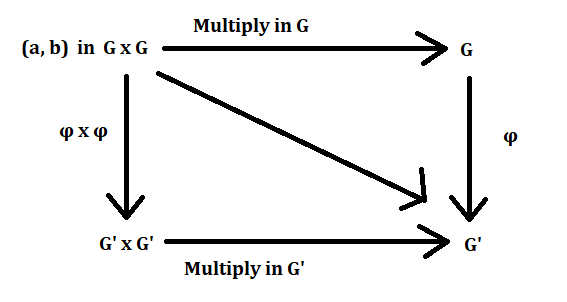
\includegraphics[scale=0.7]{assets/homo_diagram.png}
\end{center}
This is known as a \emph{commutative diagram}.

\subsection{Examples of Homomorphisms}
We will now discuss some simple example of homomorphisms. 

\subsubsection{Example: Integers}
Consider the following function: 
\[c_n: (\Z, +) \to (\Z / \Z n, +)\]
Defined by: 
\[c_{n}(a) = [a]_n\]
We can say that $c_n$ is a group homomorphism since for all $a, b \in \Z$: 
\[c_{n}(a + b) = [a + b]_n = [a]_n + [b]_n = c_{n}(a) + c_{n}(b)\]

\subsubsection{Example: Function Negation}
Consider the following function: 
\[f: (\Z, +) \to (\Z, +)\]
Defined by: 
\[f(x) = -x\]
Then, we say that $f$ is a group homomorphism since for all $x, y \in \Z$: 
\[f(x + y) = -(x + y) = (-x) + (-y) = f(x) + f(y)\]

\subsubsection{Example: Exponential Map}
Consider the following function: 
\[\phi: (\R, +) \to (\R - \{0\}, \times)\]
Defined by: 
\[\phi(x) = e^x\]
Then, $\phi$ is a group homomorphism since for all $x, y \in \R$: 
\[\phi(x + y) = e^{x + y} = e^x \times e^y = \phi(x) \times \phi(y)\]


\subsubsection{Example: Generalized Exponential Map}
Suppose $(G, *)$ is a group and $g \in G$. Then, we can consider the following function: 
\[f: (\Z, +) \to (G, *)\]
Defined by: 
\[f(n) = g^n\]
We know that this is a group homomorphism because for every $m, n \in Z$:
\[f(m + n) = g^{m + n} = g^m * g^n = f(m) * f(n)\]

\subsubsection{Example: Logarithmic Map}
Consider the following logarithmic function: 
\[\ln: (\R_{> 0}, \times) \to (\R, +)\]
We know that this is a group homomorphism since for all $x, y \in \R_{ > 0}$: 
\[\ln(x \times y) = \ln(x) + \ln(y)\]

\subsubsection{Example: Complex Numbers}
Consider the following function: 
\[N: (\C - \{0\}, \times) \to (\R_{> 0}, \times)\]
Defined by: 
\[N(z) = |z|\]
This is a group homomorphism because for every $z \in \C - \{0\}$ and $|z| \in \R_{> 0}$:
\[|z_1 \times z_2| = |z_1| \times |z_2|\]

\subsubsection{Example: Matrices}
Define $(GL_{n}(\R), \cdot)$ be the set of invertible $n \times n$ real matrices under matrix multiplication.\footnote{From linear algebra, we know that matrix multiplication is associative, the product of two invertible $n \times n$ is invertible, and for every $a \in GL_{n}(\R)$, $a \cdot I_n = I_n \cdot a = a$ where $I_n$ is the identity matrix.} Consider the function: 
\[\theta: GL_{n}(\R) \to GL_{n}(\R)\]
Defined by\footnote{If $x$ is a matrix, then $x^T$ is the transpose of said matrix.}: 
\[\theta(x) = (x^T)^{-1}\]
We know that $\theta$ is a group homomorphism because: 
\[\theta(x \cdot y) = ((x \cdot y)^T)^{-1} = (y^T \cdot x^T)^{-1} = (x^T)^{-1} \cdot (y^T)^{-1} = \theta(x) \cdot \theta(y)\]

\subsection{Properties of Homomorphisms}
\begin{mdframed}
    \begin{proposition}
        Let $\phi: G \to G'$ be a group homomorphism. 
        \begin{enumerate}[(a)]
            \item $\phi$ maps the identity to the identity: $\phi(e_G) = e_{G'}$. 
            \item $\phi$ maps inverses to inverses; in other words, for every $a \in G$, $\phi(a^{-1}) = \phi(a)^{-1}$ where $a^{-1}$ is the inverse of $a$ in $G$ and $\phi(a)^{-1}$ is the inverse of $\phi(a)$ in $G'$. This can also be written as: 
            \[e_G = \phi(a) \phi(a^{-1})\]
            \item If $a_1, \dots, a_k$ are elements of $G$, then $\phi(a_1, \dots, a_k) = \phi(a_1) \dots \phi(a_k)$. 
        \end{enumerate}
    \end{proposition}
\end{mdframed}

The proof is as follows: 
\begin{mdframed}
    \begin{proof}
        We need to show that all three properties hold. 
        \begin{enumerate}[(a)]
            \item We note that since $e_G$ is the identity element of $G$, it follows that $e_G * e_G = e_G$. Because $\phi$ is a group homomorphism, it follows that: 
            \[\boxed{\phi(e_G * e_G)} = \phi(e_G) * \phi(e_G)\]
            Since $e_G * e_G = e_G$, it follows that $\phi(e_G * e_G) = \phi(e_G)$, so: 
            \[\phi(e_G) * \phi(e_G) = \boxed{\phi(e_G)}\]
            Thus: 
            \[\phi(e_G) * \phi(e_G) = \phi(e_G) * e_{G'}\]
            Canceling the first element in each side, we now have: 
            \[\phi(e_G) = e_{G'}\]

            \item For every $a \in G$, we know that $a * a^{-1} = e_G$. Applying $\phi$ to both sides, we have that: 
            \[\phi(a * a^{-1}) = \phi(e_G)\]
            By the first part and the fact that $\phi$ is a group homomorphism, we deduce that: 
            \[\phi(a) * \phi(a^{-1}) = e_{G'}\]
            Multiplying both sides by the inverse $\phi(a)^{-1}$ of $\phi(a)$ in $G'$, we obtain: 
            \[\phi(a)^{-1} * \phi(a) * \phi(a^{-1}) = \phi(a)^{-1} * e_H\]
            And so:
            \[\phi(a^{-1}) = \phi(a)^{-1}\]

            \item We can simply make use of induction from the definition. \qedhere
        \end{enumerate}
    \end{proof}
\end{mdframed}


\subsection{Image}
\begin{definition}{Image}{}
    The \textbf{image} of a general homomorphism $\phi: G \to G'$ is simply the image of $\phi$ as a map of sets: 
    \[\im(\phi) = \{x \in G' \mid x = \phi(a) \text{ for some } a \in G\}\]
\end{definition}
The image of $\phi$ is a subgroup of $G'$. Say $a, b \in G'$ are in the image; that is, $\exists x, y \in G$ such that $\phi(x) = a$, $\phi(y) = b$. Then: 
\[\phi(xy) = ab\]
This implies that the image has closure. The image has the identity (consider the second property in the propositions). Finally, the image has the inverse since $\phi(x^{-1}) = a^{-1}$. 

\subsection{Kernal}
\begin{definition}{Kernal}{}
    The \textbf{kernal} of a general homomorphism $\phi: G \to G'$ is the set of elements of $G$ that are mapped to the identity in $G'$: 
    \[\ker(\phi) = \{a \in G \mid \phi(a) = e_{G'}\}\]
\end{definition}
Here, the kernal of $\phi$ is a subgroup of $G$. 


\subsubsection{Example: Matrices}
For example, we have that $\phi: \det GL_n (\R) \to (\R - \{0\}, \times)$, which means that: 
\[\ker(a) = SL_n\]
Where $SL_n$ is the special linear group of $n \times n$ matrices. 











\newpage 
\section{Isomorphisms}
We now discuss isomorphisms, a special type of homomorphisms.

\subsection{Motivating Example}
Before we talk about isomorphisms, let's first talk about two motivating examples. 

\subsubsection{Motivating Example 1: Tables}
Let's suppose we are given two groups.
\begin{itemize}
    \item \underline{Group 1:} $(\Z / \Z 4, +)$. 
    \item \underline{Group 2:} $(\{1, -1, i, -i\}, \times)$
\end{itemize}
At first, these groups don't look at all related to each other. They even have completely different operations. However, they are structurally similar. 

\bigskip 

Consider the table that represents group 1:
\begin{center}
    \begin{tabular}{c|c c c c}
        $+$     & 0 & 1 & 2 & 3 \\ 
        \hline 
        0       & 0 & 1 & 2 & 3 \\
        1       & 1 & 2 & 3 & 0 \\ 
        2       & 2 & 3 & 0 & 1 \\ 
        3       & 3 & 0 & 1 & 2
    \end{tabular}
\end{center}
Now, consider the table that represents group 2: 
\begin{center}
    \begin{tabular}{c|c c c c}
        $\times$ & 1 & $i$ & $-1$ & $-i$ \\ 
        \hline 
        1        & 1 & $i$ & $-1$ & $-i$ \\ 
        $i$      & $i$ & $-1$ & $-i$ & 1 \\ 
        $-1$     & $-1$ & $-i$ & 1 & $i$ \\ 
        $-i$     & $-i$ & 1 & $i$ & $-1$
    \end{tabular}
\end{center}
One thing that should be clear (after some observation) is how the elements in both tables correspond with each other. Consider the same tables from above, now highlighted: 
\begin{center}
    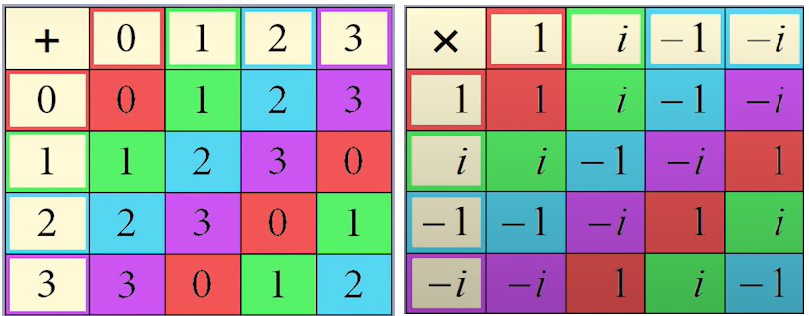
\includegraphics[scale=0.5]{assets/homo_ex.png}
\end{center}
Both tables exhibit the same patterns. They're essentially identical groups; they just use different elements and different operations. For instance, in both tables, if we combined a green element with a blue element, we get a purple element. If we combined a blue element with a blue element, we get a red element. In other words, any statement about one table can be said for the other. 

\bigskip 

We say that these two groups are \emph{isomorphic} (equal form). 

\subsubsection{Motivating Example 2: Addition Table}
Consider the following addition table of $(\Z / \Z_3, +)$.
\begin{center}
    \begin{tabular}{c|c c c}
        $+$     & $[0]_3$ & $[1]_3$ & $[2]_3$ \\ 
        \hline 
        $[0]_3$ & $[0]_3$ & $[1]_3$ & $[2]_3$ \\
        $[1]_3$ & $[1]_3$ & $[2]_3$ & $[0]_3$ \\
        $[2]_3$ & $[2]_3$ & $[0]_3$ & $[1]_3$ 
    \end{tabular}
\end{center}
Now, consider the Roman numbers: 
\begin{center}
    \begin{tabular}{c|c c c}
        $+$     & 0 & I & II \\ 
        \hline 
        0       & 0 & I & II \\ 
        I       & I & II & 0 \\ 
        II      & II & 0 & 1
    \end{tabular}
\end{center}
It's clear that both of these are the same groups, only written with different symbols. We only need a \emph{translator} to tell us which one is which. What is a translator (in the context of a group)? It should be a \emph{bijection} which preserves the operation table. Notice that preserving the operation table simply means that it should be a group homomorphism. This brings us to the definition of group isomorphism. 


\subsection{Definition of Isomorphism}
\begin{definition}{Isomorphism}{}
    An \textbf{isomorphism} of two groups $(G, *)$ and $(G', \cdot)$ is a \emph{homomorphism}: 
    \[\phi: G \to G'\]
    Which is \underline{bijective} (on sets). If there is a isomorphism $\phi: G \to G'$, we say that $G$ is isomorphic to $G'$. 
\end{definition}

\subsection{Inverse of Isomorphism}
Let $\phi^{-1}: G' \to G$ be the inverse function. Then, $\phi^{-1}$ is also a homomorphism. In other words: 
\[\forall a, b \in G', \phi^{-1}(a \cdot b) = \phi^{-1}(a) * \phi^{-1}(b)\]
Let $x = \phi^{-1}(a)$ and $y = \phi^{-1}(b)$ so that: 
\[\phi(x * y) = \phi(x) \cdot \phi(y)\]
Which follows that: 
\[x * y = \phi^{-1}(a) * \phi^{-1}(b) = \phi^{-1}(\phi(x) \cdot \phi(y)) = \phi^{-1}(a \cdot b)\]

\subsection{Pictorial Interpretation}
A pictorial interpretation can be seen as follows: 
\begin{center}
    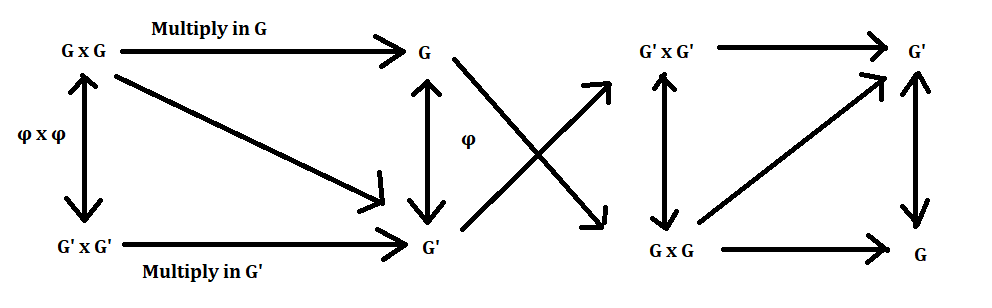
\includegraphics[scale=0.6]{assets/iso_diagram.png}
\end{center}

\subsection{Properties of Isomorphisms}
We say that $G$ and $G'$ are isomorphism if there exists some isomorphism between them. Any \emph{purely structural} property of a group is isomorphism-stable in the sense that if $G$ and $G'$ are isomorphic and $G$ has a property, then $G'$ does as well. 

\bigskip 

Some examples of structural properties include: 
\begin{itemize}
    \item Being finite. 
    \item Having order $n$ for any $n$. 
    \item Being cyclic. 
    \item Being abelian/commutative. 
    \item Number of leements of a given order. 
\end{itemize}

\textbf{Remarks:}
\begin{itemize}
    \item $\Z / \Z 6$ is not isomorphic to $S_3$ because $\Z / \Z 6$ is commutative but $S_3$ is not. 
    \item Any two cyclic groups of the same order are isomorphic. 
\end{itemize} 

\subsection{Examples of Non-Cyclic Isomorphisms}
The following examples are isomorphic to each other: 
\begin{itemize}
    \item The Klein 4-Group: 
    \begin{center}
        \begin{tabular}{c|c|c|c|c}
                & 1 & $a$ & $b$ & $c$ \\ 
            \hline 
            1   & 1 & $a$ & $b$ & $c$ \\ 
            $a$ & $a$ & 1 & $c$ & $b$ \\ 
            $b$ & $b$ & $c$ & 1 & $a$ \\ 
            $c$ & $c$ & $b$ & $a$ & 1
        \end{tabular}
    \end{center}

    \item $H \subseteq S_4$: 
    \[\left\{1, (12)(34), (13)(24), (14)(23)\right\}\]

    \item $(\Z / \Z 8 - \{0\}, \times)$
    \[\{1 \Mod{8}, 3 \Mod{8}, 5 \Mod{8}, 7 \Mod{8}\}\]
\end{itemize}
Even though these examples are completely different, they are isomorphic (they are very similar in \emph{structure}). 










\newpage 
\section{Equivalence Relations}
We will briefly talk about equivalence relations, which are particularly important for near-future topics like cosets.

\bigskip 

\textbf{Note:} A lot of the notes here was taken from Professor Golsefidy's Math 103A notes. 

\subsection{Definition}
Let $S$ be a non-empty set. Then, a \textbf{relation} over $S$ is a subset $R$ of $S \times S$. If $(x, y) \in R$, we say that $x$ is $R$-related to $y$ and write $x R y$. 

\bigskip 

So, for these relations, we should think about inequalities equalities, or congruences between integers. 

\bigskip 

Suppose $R$ is a relation over $S$. Then:
\begin{itemize}
    \item $R$ is called \textbf{reflexive} if $\forall x \in S$, $x R x$. That is, every $x \in S$ is related to itself. 
    \item $R$ is called \textbf{symmetric} if $\forall x, y \in S$, $x R y \implies y R x$. In other words, if $x$ is related to $y$, is $y$ related to $x$? 
    \item $R$ is called \textbf{transitive} if $\forall x, y, z \in S$, $x R y$ and $y R z$ implies that $x R z$. 
\end{itemize}

\begin{definition}{Equivalence Relation}{equivRel}
    An \textbf{equivalence relation} on a set $S$ is a relation that holds between certain pairs of elements of $S$. We may write it as $a \sim b$ and speak of it as \emph{equivalence} of $a$ and $b$ (or simply, $a$ is equivalent to $b$). An equivalence relation is required to be: 
    \begin{itemize}
        \item \underline{Reflexive:} For all $a$, $a \sim a$. 
        \item \underline{Symmetric:} $\forall a, b \in S$, if $a \sim b$, then $b \sim a$. 
        \item \underline{Transitive:} $\forall a, b, c \in S$, if $a \sim b$ and $b \sim c$, then $a \sim c$. 
    \end{itemize}
\end{definition}

\textbf{Remarks:}
\begin{itemize}
    \item An equivalence relation is essentially an equality with respect to a certain measurement. In life, we often measure things or people with respect to properties (for example, scores or ratings). So, when we want to compare things, we pick a certain property and then, \emph{from that point of view}, determine whether these things are equal. In this regard, equivalence relations are exactly equalities. 
    \item Another way we can think of an equivalence relation is through a function: 
    \[S \times S \to \{\text{true}, \text{false}\}\]
\end{itemize} 

\subsubsection{Example: Relations}
Suppose $X$ and $Y$ are two non-empty sets and $f: X \to Y$ is a function. Let $\sim$ be the following relation over $X$:
\[\forall x_1, x_2 \in X \quad x_1 \sim x_2 \iff f(x_1) = f(x_2)\]
Then, $\sim$ is an equivalence relation\footnote{Another way of interpreting this statement is as follows: $x_1$ is in relation to $x_2$ precisely when $f(x_1) = f(x_2)$. The claim here, then, is that this is an equivalence relation.}.

\begin{mdframed}
    \begin{proof}
        We determine if an relation is an equivalence relation if it satisfies the three properties mentioned above.
        \begin{itemize}
            \item \underline{Reflexivity:}
            \[\forall x \in X, f(x) = f(x) \implies x \sim x\]
    
            \item \underline{Symmetric:}
            \[x_1 \sim x_2 \implies f(x_1) = f(x_2) \implies f(x_2) = f(x_1) \implies x_2 \sim x_1\]
    
            \item \underline{Transitive:}
            We know that:
            \[\forall x_1, x_2 \in X \qquad x_1 \sim x_2 \implies f(x_1) = f(x_2)\]
            We also know that:
            \[\forall x_2, x_3 \in X \qquad x_2 \sim x_3 \implies f(x_2) = f(x_3)\]
            It follows that if $f(x_1) = f(x_2)$ and $f(x_2) = f(x_3)$, then $f(x_1) = f(x_3)$ and thus, $x_1 = x_3$. Namely, $x_1 \sim x_2$ and $x_2 \sim x_3$, then $x_1 \sim x_3$. 
        \end{itemize}
        It follows that this is an equivalence relation. 
    \end{proof}
\end{mdframed}

\subsection{Equivalence Relation Partitions}
Recall that $P$ is called a \textbf{partition} of a non-empty set $X$ if:
\begin{itemize}
    \item \underline{Subsets:} $P$ consists of non-empty subsets of $X$. 
    \item \underline{Disjointness:} $A, B \in P$ and $A \neq B \implies A \cap B = \emptyset$. In other words, the subsets are disjoint. 
    \item \underline{Covering:} $\forall x \in X$, $\exists A \in P$ such that $x \in A$. In other words, every element in $X$ will be in one of the subsets. Alternatively, $\bigcup_{A \in P} A = X$. 
\end{itemize}

\textbf{Remark:}
\begin{itemize}
    \item As mentioned, $P$ is a set of sets. For instance, if we have $X = \{1, 2, 3\}$, one possible $P$ is $P = \{\{1\}, \{2, 3\}\}$.
    \item Below is a visual diagram of what a partition may look like.
\end{itemize}
\begin{center}
    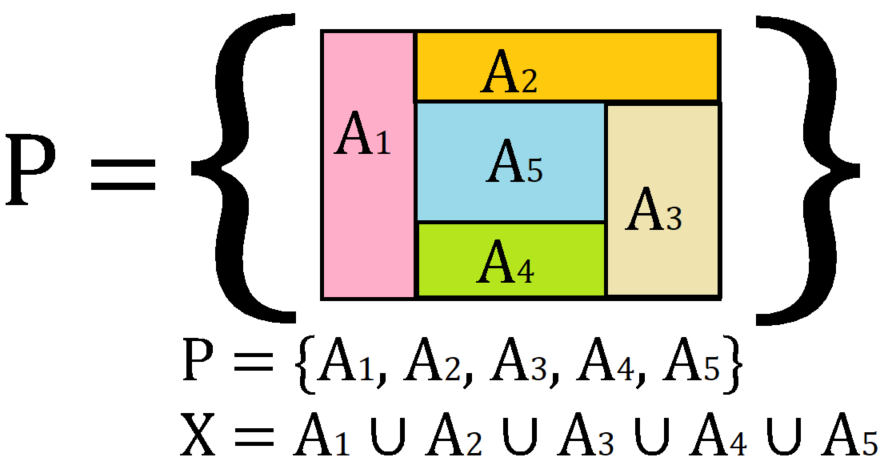
\includegraphics[scale=0.4]{assets/partition.PNG}
\end{center}

Suppose $P$ is a partition of $X$. Then, we can get a classification function from $X$ to $P$:
\[X \to P\]
\[x \mapsto [x]_P\]
Here, $[x]_P$ is the unique element of $P$ which contains $x$. In other words, if we refer to the above diagram, we can think of $[x]_P$, a set, as one of the sets $A_1$, $A_2$, $A_3$, $A_4$, or $A_5$ which contains $x$. So, we can think of this function as saying that every $x \in X$ belongs to one of the sets $[x]_P$. 

\bigskip 

Notice that, because of the \textbf{covering} condition, $x$ is contained in some element of $P$; additionally, because of the \textbf{disjointness} condition, $x$ is in an unique element of $P$ (i.e. it is in \underline{one} of the sets which is in $P$). So, it follows that the function is well-defined. 

\bigskip 

By the previous example, $x \sim_P y \iff [x]_P = [y]_P$ is an equivalence relation. So, we obtain the following lemma. 
\begin{lemma}{}{}
    Suppose $P$ is a partition of a non-empty set $X$. For $x, y \in X$, $x \sim y$ if $x$ and $y$ are in the same element of $P$. Then, $\sim$ is an equivalence relation.
\end{lemma}
\textbf{Remark:} Essentially, what this lemma is saying is that if $x \sim y$, then both $x$ and $y$ are in the same set which is in $P$. In other words, if we refer to the above diagram again, we can think of this situation as saying that both $x$ and $y$ are in \underline{one} of $A_1$, $A_2$, $A_3$, $A_4$, or $A_5$. The diagram below complements the proof.

\begin{center}
    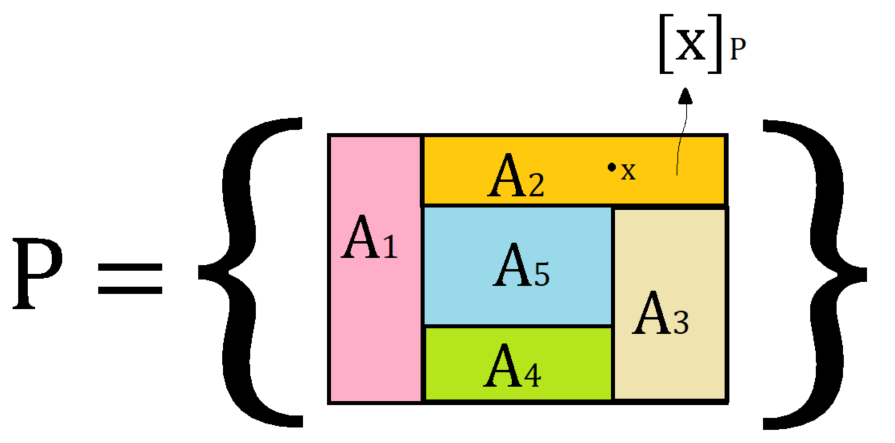
\includegraphics[scale=0.30]{assets/partition_x.PNG}
\end{center}

\begin{mdframed}
    \begin{proof}
        For $x \in X$, let $[x]_P$ to be the unique element of $P$ which contains $x$. So, $x \mapsto [x]_P$ is a function from $X \to P$. By the previous example, $x \sim y \iff [x]_p = [y]_p$ is an equivalence relation over $X$. Notice that this means $x \sim y$ exactly when $x$ and $y$ are in the same element of $P$. 
    \end{proof}
\end{mdframed}

\subsection{Equivalence Relation Classes}
Now, suppose that $\sim$ is the equivalence relation over a non-empty set $X$, we can partition $X$ with respect to $\sim$. 

\bigskip 

For $x \in X$, we let $[x] = \{y \in X \mid y \sim x\}$ (all the elements that are $\sim$-related to $x$).\footnote{So, it's obvious that $[x] \subseteq X$.} We call $[x]$ the \textbf{equivalence class of $x$ with respect to $\sim$}. When $x \sim y$, we can say that $x$ is equivalent to $y$ with respect to $\sim$. 

\begin{proposition}
    Suppose $\sim$ is an equivalence relation over a non-empty set $X$. Then, $\{[x] \mid x \in X\}$ is a partition of $X$. 
\end{proposition}
This proposition is essentially asking us to show the following properties: 
\begin{itemize}
    \item Covering: Every element of this set belongs to one of these equivalence classes. 
    \item Disjointness: If we pick two equivalence classes, they do not intersect.
\end{itemize}
The following lemma follows from this proposition.
\begin{lemma}{}{}
    \[x \sim y \iff [x] = [y]\]
\end{lemma}
\begin{mdframed}
    \begin{proof}
        We want to show that $[x] = [y] \implies x \sim y$. Recall that the equivalence class of $x$ ($[x]$) and the equivalence class of $y$ ($[y]$) are \emph{sets} and, in particular, we know that $[x]$ consists of all elements that are related to $x$, including $x$. Since $\sim$ is reflexive, we know that:
        \[x \sim x \implies x \in [x]\]
        But, since $[x] = [y]$, then it follows that $x \in [y] \implies x \sim y$. Thus, $[x] = [y] \implies x \sim y$. 
        
        \bigskip 
    
        To show that $x \sim y \implies [x] = [y]$, we need to show equality of sets $[x] = [y]$. This means that it is necessary and sufficient to prove $[x] \subseteq [y]$ and $[y] \subseteq [x]$.
        \begin{itemize}
            \item To prove $[x] \subseteq [y]$, we let $z \in [x]$. This means that $z \sim x$. However, since $x \sim y$, by transitivity, it follows that $y \sim z$, which implies that $z \in [y]$. Hence, $[x] \subseteq [y]$. 
            \item We note that $x \sim y \implies y \sim x$ by symmetry. Therefore, by the first bullet point, $[y] \subseteq [x]$.
        \end{itemize} 
        So, it follows that $x \sim y \implies [x] = [y]$. 
    \end{proof}
\end{mdframed}

Now that we proved the lemma, we can now prove the proposition. 
\begin{mdframed}
    \begin{proof}
        As mentioned, we need to show that the covering and disjointness properties exist in this partition.
        \begin{itemize}
            \item \underline{Covering:} $\forall x \in X$, we know that $x \sim x$ by the reflexive property (since $\sim$ is an equivalence relation). Thus, it follows that $x \in [x]$. This means that $x$ is related to $x$ and $x$ is an equivalence class of $x$, so every element in $X$ belongs to one of the equivalence classes. This implies that the $[x]$ sets are non-empty subsets and cover $X$.
            \item \underline{Disjointness:} Suppose $z \in [x] \cap [y]$ (both equivalence classes are not disjoint). We need to show that they are equal. We know that:
            \[z \in [x] \cap [y] \implies z \in [x] \implies z \sim x \implies [z] = [x]\]
            \[z \in [x] \cap [y] \implies z \in [y] \implies z \sim y \implies [z] = [y]\]
            Where the last two steps came from the lemma. Then, putting these two together, we have:
            \[[z] = [x] \text{ and } [z] = [y] \implies [x] = [y]\]
            We showed that $[x] \cap [y] \neq \emptyset \implies [x] = [y]$, the contrapositive of the disjointness property. 
        \end{itemize}
        Thus, the proof is complete. 
    \end{proof}
\end{mdframed}

\end{document}